\chapter{Background}
\label{cha:techstack}

Before we describe the project, we need to know what we are talking about. In particular, these are the software and strongly used in the project:  
\begin{itemize}
    \item ROS2
    \item Gazebo
    \item \acrfull{rviz}
    \item \acrfull{nav2}
    \item Docker
\end{itemize}

\section{\acrshort{ros}2}

\begin{wrapfigure}{l}{0.2\textwidth}
    
\includegraphics[width=0.2\textwidth]{images/foxy}
\end{wrapfigure}

\textit{\acrshort{ros}2, which stands for Robot Operative System 2, is a set of software libraries and tools for building robot applications.}\cite{ros2desc} On it, each process is a node and each node has the ability to talk to others thanks to some communication channels called topics, using the publish/subscribe model.

This version of \acrshort{ros}2, called \textbf{Foxy Fitzroy}, was used because it is possible to integrate the \textit{plansys2} libraries used for planning.

Thanks to \acrshort{ros} \textit{hardware abstraction, low-level device control, implementation of commonly-used functionality, message-passing between processes, and package management}\cite{ros2help}, the developer can ignore specific hardware details and software implementations and focus only on the application itself. 

This means that running a \acrshort{ros} node on your own computer is the same as running it on a robot, as long as you are use the same \acrfull{os} (only \textbf{Ubuntu 20.04}) and the same external devices, if you are not simulating them.

\section{Gazebo}
\label{sec:gazebo}

\begin{wrapfigure}{r}{0.25\textwidth}
    
\includegraphics[width=0.25\textwidth]{images/gazebo}
\end{wrapfigure}

Gazebo is a simulation suite. It lets you create and simulate things with the bundled physic and render engines, alongside a variety of sensors.

It comes as a standalone software, but thanks to its interfaces it is possible to integrate it with \acrshort{ros}2, using several packages developed for this purpose: in this way you can simulate both robots and the environments in which they operate, before actually moving to the real world, or to test your last modifications even if you are somewhere other than the real robot location.

With sensors and plugins you are able to simulate lasers (e.g. lidars), cameras (e.g. depth cameras), IMUs, and GPS receivers, or even differential drive and joints state.

\section{\acrfull{rviz}}

\begin{wrapfigure}{l}{0.25\textwidth}
    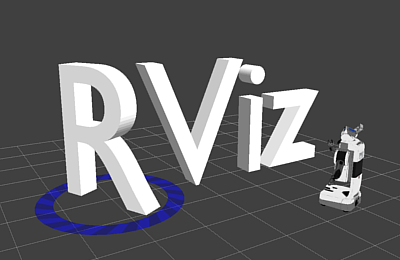
\includegraphics[width=0.25\textwidth]{images/rviz}
\end{wrapfigure}

\acrshort{rviz}, is a visualization tool for \acrshort{ros}: you can view sensors, robots, and the environment; in general, you can see the actual state of the \acrshort{ros} system. In this project it was used to set initial position of the robot on the map, see the boundaries of the room and the obstacles, and view the path that the robot is currently following to reach the goal, which could be specified graphically (manually) or from other nodes (automatically). 

\section{\acrfull{nav2}}

\begin{wrapfigure}[8]{r}{0.1\textwidth}
    
\includegraphics[width=0.1\textwidth]{images/nav2_logo}
\end{wrapfigure}

The Navigation Stack is a collection of \acrshort{ros}2 packages that provide useful tools for navigating your robot: path planning, localization, obstacle avoidance, recovery from collisions, mapping and others\footnote{A detailed description can be found in \autoref{cha:navigation}}. These packages have been used as the basis for this project: in this way you do not have to worry about the navigation algorithms, just pass the sensor information, and they will do the rest; moreover, you can use the provided interfaces to customize and automate the entire navigation process.

It can be thought of as a template for navigation systems with a generic configuration, and thanks to \acrshort{ros}, you can easily set the desired parameters for each node with a YAML file: this will be analyzed when you start the navigation stack and the nodes will be configured accordingly.

\section{Docker}
  
\begin{wrapfigure}[3]{r}{0.15\textwidth}
    
\includegraphics[width=0.15\textwidth]{images/docker}
\end{wrapfigure}
  
Docker is a platform that allows you to separate applications using an isolated environment called container. It also gives you the possibility to run multiple containers at once. Docker was used in this project for the following reasons:
  
\begin{itemize}
    \item \textbf{separate} this project workspace from all others, to \textbf{avoid conflicts};
    \item keep the \textbf{same} workspace for \textbf{each device} (real robot or simply a computer);
    \item permit development on any device not necessarily running \textbf{Ubuntu 20.04} (required from \acrshort{ros}2) as \acrshort{os} system.
\end{itemize}

To be more precise, inside a Dockerfile\footnote{A file containing instructions on how to build an image, used as a starting point when launching a container, with the desired packages and configurations}, after pulling the data from a pre-built image\cite{dockerimage}, all the commands needed to install the missing packages have been typed.

Using just an image is \textbf{not enough}, because you need to set up and start your project \textbf{manually} each time: a plugin called \code{docker compose} helps in this process. It lets you specify \textbf{services} (i.e. custom actions to perform), which  will be automatically executed in separate containers (using the image defined above as a starting point), in an order that meets their mutual dependencies.